\documentclass[a4paper,12pt]{report}
\usepackage[T2A]{fontenc}
\usepackage[utf8]{inputenc}
\usepackage[english,russian]{babel}
\usepackage{graphicx}
\usepackage{wrapfig}
\usepackage{mathtext} 				% русские буквы в фомулах
\usepackage{amsmath,amsfonts,amssymb,amsthm,mathtools} % AMS
\usepackage{icomma} % "Умная" запятая: $0,2$ --- число, $0, 2$ --- перечисление
\usepackage{capt-of}
\usepackage{appendix}
\usepackage{multirow}
\usepackage{hyperref}
\usepackage{floatrow}
\usepackage[left=2cm,right=2cm,
    top=2cm,bottom=2cm,bindingoffset=0cm]{geometry}
\usepackage{multicol} % Несколько колонок
\usepackage{gensymb}
\title{Отчёт по лабораторной работе №4.5.2. 

Интерференция лазерного излучения.}
\author{Плюскова Н.А. Б04-004 }
\date{\today}
\begin{document}
\maketitle
\section*{1. Аннотация}
В работе требовалось настроить систему, изучить характер поляризации, исследовать зависимость видности интерференционной картины от разности хода интерферирующих лучей и их поляризации.

\section*{2. Теоретические сведения}
\subsection*{Гелий-неоновый лазер}
Лазер представляет собой интерферометр Фабри-Перо -- газовую трубку с двумя параллельными зеркалами по обе стороны. В лазере длиной $L$ для излучения вдоль оси для резонансных частот выполняется
\begin{equation}
f_m = \dfrac{c}{\lambda_m} = \dfrac{mc}{2L}.
\end{equation}
Условие генерации может выполняться для сразу нескольких колебаний с частотами $f_m$, расположенными в диапазоне генерации $2\Delta F$. В этом случае генерируется несколько волн -- \textit{мод}, межмодовое расстояние для которых
\begin{equation}
\Delta \nu = f_{m+1} - f_m = \dfrac{c}{2L}.
\end{equation}
Число мод можно оценить как: 
\begin{equation}
N \approx 1 + \dfrac{2\Delta F}{\Delta \nu}.
\end{equation}
\subsection*{Видность}
Видность интерференционной картины -- параметр, определяемый формулой:
\begin{equation}
\gamma = \dfrac{I_{max} - I_{min}}{I_{max} + I_{min}},
\end{equation}
где $I_{max}$, $I_{min}$ -- максимальная и минимальная интенсивности света интерференционной картины вблизи выбранной точки. Разобьём его на произведение функций параметров установки
$$\gamma = \gamma_1 \gamma_2 \gamma_3.$$

Здесь $\gamma_1$ отвечает за соотношение интенсивности интерферирующих волн:
\begin{equation}
\gamma_1 = \dfrac{2\sqrt{\delta}}{1+\delta},
\end{equation}
где $\delta = \frac{B_m^2}{A_m^2}$, $A_m$ и $B_m$ -- амплитуды волн. Параметр $\delta$ определяется устройством разделения волн.

\begin{center}
    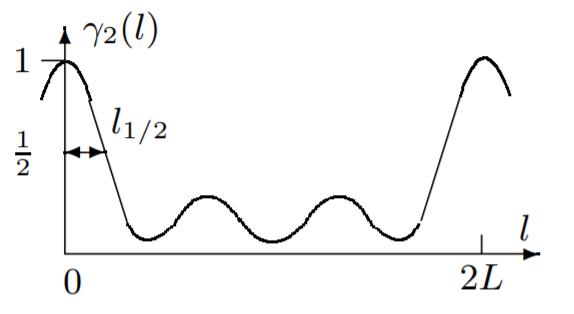
\includegraphics[scale = 1]{1.png}
    \captionof{figure}{Зависимость $\gamma_2 = \gamma_2(l)$}
\end{center}

Функция $\gamma_2$ отвечает за влияние разности хода и спектрального состава волн,

$$
\gamma_2 = \dfrac{\sum\limits_n A^2_n \cos \frac{2\pi \Delta \nu n l}{c}}{\sum\limits_n A_n^2},
$$
где $l$ -- разность хода, $\Delta \nu$ -- спектральный состав излучения, $A_n^2$ -- интенсивности мод. В непрерывном пределе получим:
$$
\gamma_2 = e^{-\left(\frac{\pi \Delta F l}{c}\right)^2}
$$
-- для гауссовой линии излучения с полушириной $\Delta F$ получили гауссову зависимость $\gamma_2 = \gamma_2(l)$ с полушириной 
\begin{equation}
l_{1/2} = \dfrac{c}{\pi \Delta F}\sqrt{\ln 2} \approx \dfrac{0.26 c}{\Delta F}.
\end{equation}
Последняя функция $\gamma_3$ отвечает за разность в поляризации. Если $\alpha$ -- угол между плоскостями поляризаций волн, то
\begin{equation}
\gamma_3 = |\cos \alpha|.
\end{equation}
\section*{3. Экспериментальная установка}

В работе используется интерферометр Майкельсона (Рис. 2а). Луч лазера, отражённый от зеркала З и прошедший через параллелепипед Френеля (ПФ), делится делительной призмой ДП на два луча. Первый проходит блок $\text{Б}_1$ с поляроидом $\text{П}_1$ и зеркалом $\text{З}_1$, приклеенным к пьезокерамике, которая может совершать малые колебания вдоль луча, с возможность изменения угла наклона зеркала. Второй проходит блок $\text{Б}_2$ с линзой Л, поляроидом $\text{П}_2$ и зеркалом $\text{З}_2$ в фокальной плоскости линзы, чтобы выходящий луч, в отличие от первого, был параллелен входящему. Оба луча, проходя ДП, попадают на сферическое зеркало $\text{З}_3$ и интерферируют на экране. Интенсивность света считывается фотодиодом на осциллограф через щель, параллельную интерференционным полосам, в центре экрана. На экране осциллографа наблюдаются колебания с изменяющимся периодом, так как на пьезокерамику подаются напряжение, из-за чего её длина колеблется.

\begin{figure}[h]
\begin{minipage}[h]{0.49\linewidth}
\center{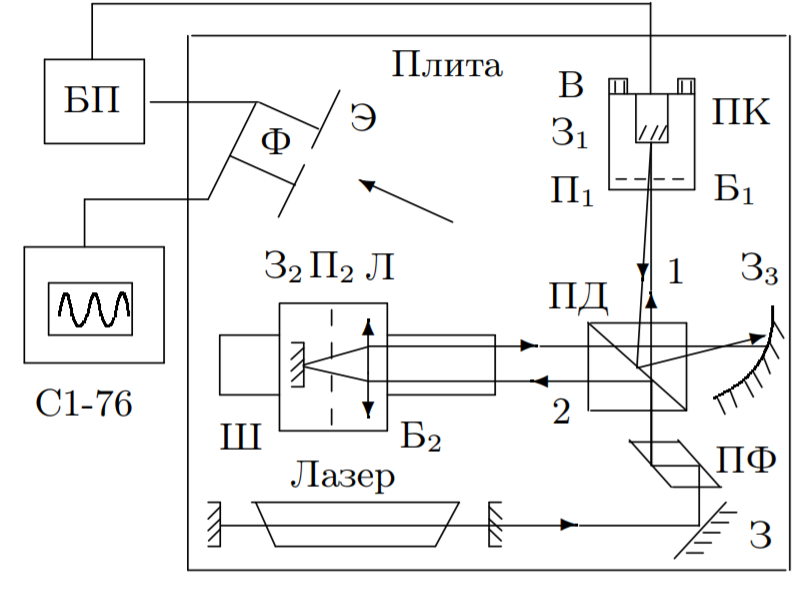
\includegraphics[width=1\linewidth]{2.png} \\ а)}
\end{minipage}
\hfill
\begin{minipage}[h]{0.49\linewidth}
\center{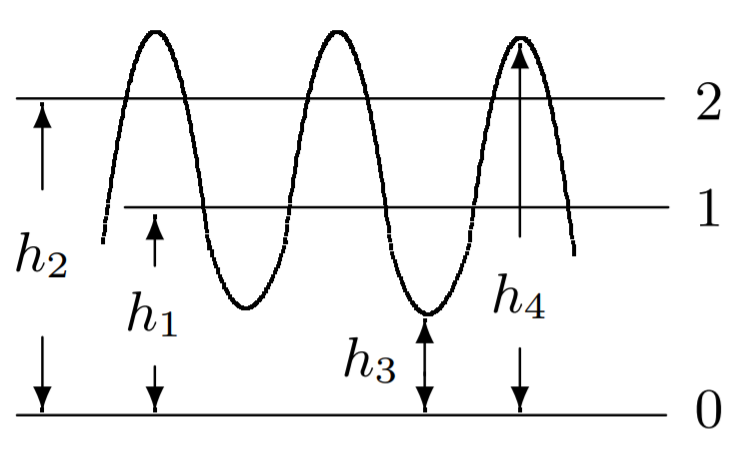
\includegraphics[width=1\linewidth]{3.png} \\б)}
\end{minipage}
\caption{а) Схема установки; б) Осциллограмма сигналов фотодиода}
\label{ris:image1}
\end{figure}


По картине на экране осциллографа можно определить параметры видимости по следующим формулам:
\begin{equation}
\delta = \dfrac{h_1}{h_2},
\end{equation}
\begin{equation}
\gamma = \dfrac{h_4 - h_3}{h_4 + h_3},
\end{equation}
Здесь 0 -- уровень при отсутствии лучей, 1 и 2 -- при закрытии одного из них. Используя $\delta$, можно рассчитать $\gamma_1$ по формуле (5).\\ 
При условии одинаковой поляризации лучей ($\alpha = 0$):
\begin{equation}
\gamma_2 = \dfrac{\gamma}{\gamma_1}.
\end{equation}
Если же разность хода отсутствует ($l = 0$), то
\begin{equation}
\gamma_3 = \dfrac{\gamma}{\gamma_1}.
\end{equation}
\section*{4. Ход работы}
\subsection*{4.1 Изучение характера поляризации}
Измерим h1 - h4 для исследования зависимости видности от поляризации (при этом считаем, что разность хода равна 0):
\begin{table}[H]
\begin{center}
\caption{Зависимость видности от угла поворота поляроида при нулевой разности хода}
\begin{tabular}{|p{0.39cm}|p{0.6cm}|p{0.6cm}|p{0.6cm}|p{0.6cm}|c|c|c|c|c|c|c|c|c|}
\hline
$\alpha$ & h1, дел & h2, дел & h3, дел & h4, дел & $\sigma_h$, дел           & $\gamma$ & $\sigma_{\gamma}$ & $\delta$ & $\sigma_{\delta}$ & $\gamma_{1}$ & $\sigma_\gamma_{1}$ & $\gamma_{3}$ & $\sigma_{\gamma_{3}}$ \\ \hline
$0^{\circ}$     & 12      & 6,8     & 2       & 35      & \multirow{10}{*}{0,05} & 0,89  & 0,01        & 1,76  & 0,02        & 0,96         & 0,01               & 0,93         & 0,02               \\ \cline{1-5} \cline{7-14} 
$10^{\circ}$    & 12      & 6,8     & 2,1     & 35      &                        & 0,89  & 0,01        & 1,76  & 0,02        & 0,96         & 0,01               & 0,92         & 0,02               \\ \cline{1-5} \cline{7-14} 
$20^{\circ}$    & 11      & 6,9     & 2       & 33      &                        & 0,89  & 0,01        & 1,59  & 0,02        & 0,97         & 0,01               & 0,91         & 0,02               \\ \cline{1-5} \cline{7-14} 
$30^{\circ}$    & 9,2     & 6,5     & 2       & 30      &                        & 0,88  & 0,01        & 1,42  & 0,02        & 0,99         & 0,01               & 0,89         & 0,02               \\ \cline{1-5} \cline{7-14} 
$40^{\circ}$    & 7,5     & 6,5     & 2,8     & 26      &                        & 0,81  & 0,01        & 1,15  & 0,02        & 1,00         & 0,01               & 0,81         & 0,02               \\ \cline{1-5} \cline{7-14} 
$50^{\circ}$    & 5,8     & 6,6     & 3,2     & 21,8    &                        & 0,74  & 0,01        & 0,88  & 0,01        & 1,00         & 0,02               & 0,75         & 0,02               \\ \cline{1-5} \cline{7-14} 
$60^{\circ}$    & 5       & 6,5     & 4,5     & 19      &                        & 0,62  & 0,01        & 0,77  & 0,01        & 0,99         & 0,02               & 0,62         & 0,02               \\ \cline{1-5} \cline{7-14} 
$70^{\circ}$    & 3       & 6,5     & 5,3     & 19      &                        & 0,56  & 0,01        & 0,46  & 0,01        & 0,93         & 0,02               & 0,61         & 0,02               \\ \cline{1-5} \cline{7-14} 
$80^{\circ}$    & 2,1     & 6,6     & 6,5     & 12      &                        & 0,30  & 0,01        & 0,32  & 0,01        & 0,86         & 0,03               & 0,35         & 0,02               \\ \cline{1-5} \cline{7-14} 
$90^{\circ}$    & 2       & 6,5     & 8       & 10,1    &                        & 0,12  & 0,01        & 0,31  & 0,01        & 0,85         & 0,03               & 0,14         & 0,01               \\ \hline
\end{tabular}
\end{center}
\end{table}

Рассчитаем коэффициент $ \gamma_3$, и построим графики $ \gamma_3(\alpha) $, $ \gamma_3(\cos\alpha) $ и $ \gamma_3(\cos^2\alpha) $:

\begin{figure}[H]
\begin{minipage}[h]{0.49\linewidth}
\center{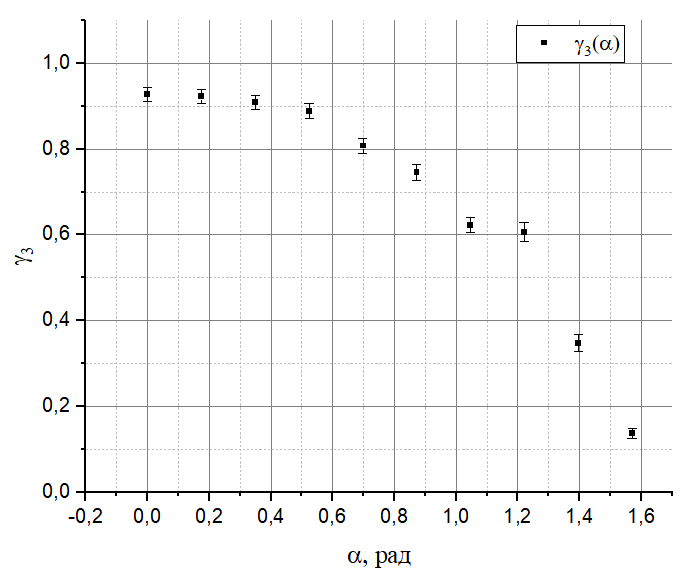
\includegraphics[width=1\linewidth]{gamma3(alpha).png} \\ а)}
\end{minipage}
\hfill
\begin{minipage}[H]{0.49\linewidth}
\center{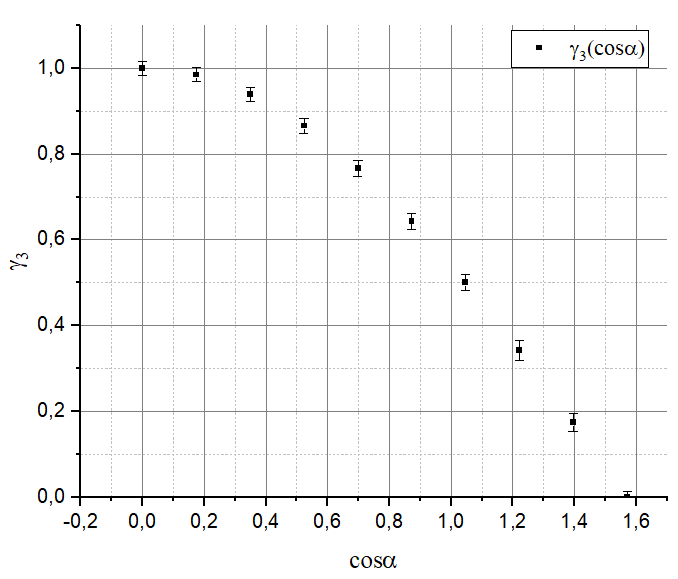
\includegraphics[width=1\linewidth]{gamma3(cos(alpha)).png} \\б)}
\end{minipage}
\caption{Зависимости а) $ \gamma_3(\alpha) $; б) $ \gamma_3(\cos\alpha) $}
\label{ris:image1}
\end{figure}

\begin{center}
    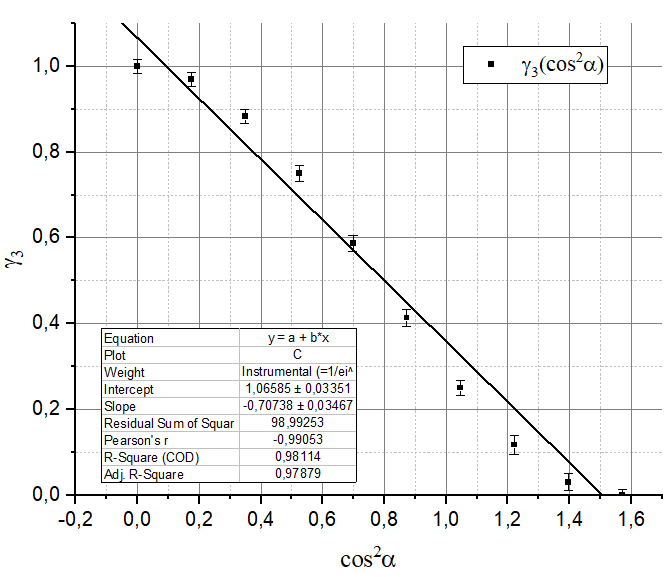
\includegraphics[width =0.8 \linewidth]{gamma3(cos^2(alpha)).png}
    \captionof{figure}{Зависимость $ \gamma_3(\cos^2\alpha) $}
\end{center}

\subsection*{4.2 Измерение коэффициента видности}

Снова измерим h1-h4, но при одинаковой поляризации лучей ($\alpha$ = 0), чтобы исследовать зависимость видности от разности хода между лучами:

\begin{table}[H]
\begin{center}
\caption{Зависимость видности от разности хода между лучами при одинаковой поляризации лучей}
\begin{tabular}{|p{0.8cm}|p{0.6cm}|p{0.6cm}|p{0.6cm}|p{0.6cm}|c|c|c|c|c|c|c|c|c|}
\hline
x,см & h1, дел & h2, дел & h3, дел & h4, дел & $\sigma_h$, дел           & $\gamma$ & $\sigma_{\gamma}$ & $\delta$ & $\sigma_{\delta}$ & $\gamma_{1}$ & $\sigma_\gamma_{1}$ & $\gamma_{2}$ & $\sigma_{\gamma_{2}}$ \\\hline
10    & 8       & 10,5    & 6       & 30      & \multirow{32}{*}{0,05} & 0,67  & -        & 0,76  & 0,01        & 0,99         & 0,01               & 0,67         & 0,01               \\ \cline{1-5} \cline{7-14} 
11    & 8       & 9       & 5       & 29      &                        & 0,71  & 0,01        & 0,89  & 0,01        & 1,00         & 0,01               & 0,71         & 0,01               \\ \cline{1-5} \cline{7-14} 
12    & 8       & 8       & 3,5     & 28      &                        & 0,78  & 0,01        & 1,00  & 0,01        & 1,00         & 0,01               & 0,78         & 0,02               \\ \cline{1-5} \cline{7-14} 
13    & 8       & 9       & 4       & 30      &                        & 0,76  & 0,01        & 0,89  & 0,01        & 1,00         & 0,01               & 0,77         & 0,01               \\ \cline{1-5} \cline{7-14} 
14    & 8       & 7       & 2,8     & 27      &                        & 0,81  & 0,01        & 1,14  & 0,02        & 1,00         & 0,01               & 0,81         & 0,02               \\ \cline{1-5} \cline{7-14} 
15    & 8       & 5       & 2       & 23      &                        & 0,84  & 0,01        & 1,60  & 0,03        & 0,97         & 0,02               & 0,86         & 0,02               \\ \cline{1-5} \cline{7-14} 
16    & 8       & 7,5     & 2,1     & 27,5    &                        & 0,86  & 0,01        & 1,07  & 0,01        & 1,00         & 0,01               & 0,86         & 0,02               \\ \cline{1-5} \cline{7-14} 
17    & 8       & 2       & 3,5     & 16      &                        & 0,64  & 0,01        & 4,00  & 0,13        & 0,80         & 0,03               & 0,80         & 0,04               \\ \cline{1-5} \cline{7-14} 
18    & 15      & 3       & 7       & 30      &                        & 0,62  & -        & 5,00  & 0,10        & 0,75         & 0,02               & 0,83         & 0,02               \\ \cline{1-5} \cline{7-14} 
20    & 9       & 6       & 4       & 25      &                        & 0,72  & 0,01        & 1,50  & 0,02        & 0,98         & 0,01               & 0,74         & 0,02               \\ \cline{1-5} \cline{7-14} 
21    & 9,5     & 9,5     & 6       & 31      &                        & 0,68  & -        & 1,00  & 0,01        & 1,00         & 0,01               & 0,68         & 0,01               \\ \cline{1-5} \cline{7-14} 
22    & 9       & 9       & 7       & 30      &                        & 0,62  & -        & 1,00  & 0,01        & 1,00         & 0,01               & 0,62         & 0,01               \\ \cline{1-5} \cline{7-14} 
23    & 9       & 8       & 7       & 27      &                        & 0,59  & -        & 1,13  & 0,01        & 1,00         & 0,01               & 0,59         & 0,01               \\ \cline{1-5} \cline{7-14} 
24    & 9       & 7       & 8       & 24      &                        & 0,50  & -        & 1,29  & 0,02        & 0,99         & 0,01               & 0,50         & 0,01               \\ \cline{1-5} \cline{7-14} 
25    & 9       & 5       & 8       & 21      &                        & 0,45  & -        & 1,80  & 0,03        & 0,96         & 0,02               & 0,47         & 0,01               \\ \cline{1-5} \cline{7-14} 
26    & 18      & 6,2     & 16      & 33      &                        & 0,35  & -        & 2,90  & 0,03        & 0,87         & 0,01               & 0,40         & 0,01               \\ \cline{1-5} \cline{7-14} 
27    & 18      & 8       & 15,5    & 33      &                        & 0,36  & -        & 2,25  & 0,02        & 0,92         & 0,01               & 0,39         & 0,01               \\ \cline{1-5} \cline{7-14} 
28    & 18      & 1,3     & 16      & 22      &                        & 0,16  & -        & 13,85 & 0,57        & 0,50         & 0,02               & 0,31         & 0,02               \\ \cline{1-5} \cline{7-14} 
35    & 16,2    & 15      & 28      & 34      &                        & 0,10  & -        & 1,08  & 0,01        & 1,00         & 0,01               & 0,10         & 0,00               \\ \cline{1-5} \cline{7-14} 
40    & 8,5     & 9       & 14      & 20,5    &                        & 0,19  & -        & 0,94  & 0,01        & 1,00         & 0,01               & 0,19         & 0,01               \\ \cline{1-5} \cline{7-14} 
45    & 16,5    & 18,5    & 27      & 33      &                        & 0,10  & -        & 0,89  & 0,01        & 1,00         & 0,01               & 0,10         & 0,00               \\ \cline{1-5} \cline{7-14} 
50    & 16,5    & 17      & 29,5    & 36      &                        & 0,10  & -        & 0,97  & 0,01        & 1,00         & 0,01               & 0,10         & 0,00               \\ \cline{1-5} \cline{7-14} 
60    & 16,5    & 4       & 19      & 22      &                        & 0,07  & -        & 4,13  & 0,06        & 0,79         & 0,01               & 0,09         & 0,00               \\ \cline{1-5} \cline{7-14} 
65    & 15,5    & 9       & 24      & 26      &                        & 0,04  & -        & 1,72  & 0,02        & 0,96         & 0,01               & 0,04         & 0,00               \\ \cline{1-5} \cline{7-14} 
71    & 15,5    & 4,2     & 15      & 26      &                        & 0,27  & -        & 3,69  & 0,06        & 0,82         & 0,01               & 0,33         & 0,01               \\ \cline{1-5} \cline{7-14} 
72    & 15,5    & 5       & 14      & 28      &                        & 0,33  & -        & 3,10  & 0,04        & 0,86         & 0,01               & 0,39         & 0,01               \\ \cline{1-5} \cline{7-14} 
73    & 15,5    & 5       & 13,5    & 29      &                        & 0,36  & -        & 3,10  & 0,04        & 0,86         & 0,01               & 0,42         & 0,01               \\ \cline{1-5} \cline{7-14} 
74    & 15,5    & 3,5     & 12      & 27,3    &                        & 0,39  & -        & 4,43  & 0,08        & 0,78         & 0,01               & 0,50         & 0,01               \\ \cline{1-5} \cline{7-14} 
75    & 15,5    & 1       & 13      & 22      &                        & 0,26  & -        & 15,50 & 0,83        & 0,48         & 0,03               & 0,54         & 0,04               \\ \cline{1-5} \cline{7-14} 
77    & 15,5    & 1,1     & 12,2    & 22      &                        & 0,29  & -        & 14,09 & 0,69        & 0,50         & 0,03               & 0,58         & 0,04               \\ \cline{1-5} \cline{7-14} 
78    & 15,5    & 1,2     & 12      & 21,5    &                        & 0,28  & -        & 12,92 & 0,58        & 0,52         & 0,02               & 0,55         & 0,03               \\ \cline{1-5} \cline{7-14} 
79    & 15,5    & 1,1     & 12      & 23      &                        & 0,31  & -        & 14,09 & 0,69        & 0,50         & 0,03               & 0,63         & 0,04               \\ \hline
\end{tabular}
\end{center}
\end{table}

Рассчитаем коэффициент $\gamma_2$ и построим график зависимости видности $\gamma_2(x)$ от координаты блока Б2:

\begin{center}
    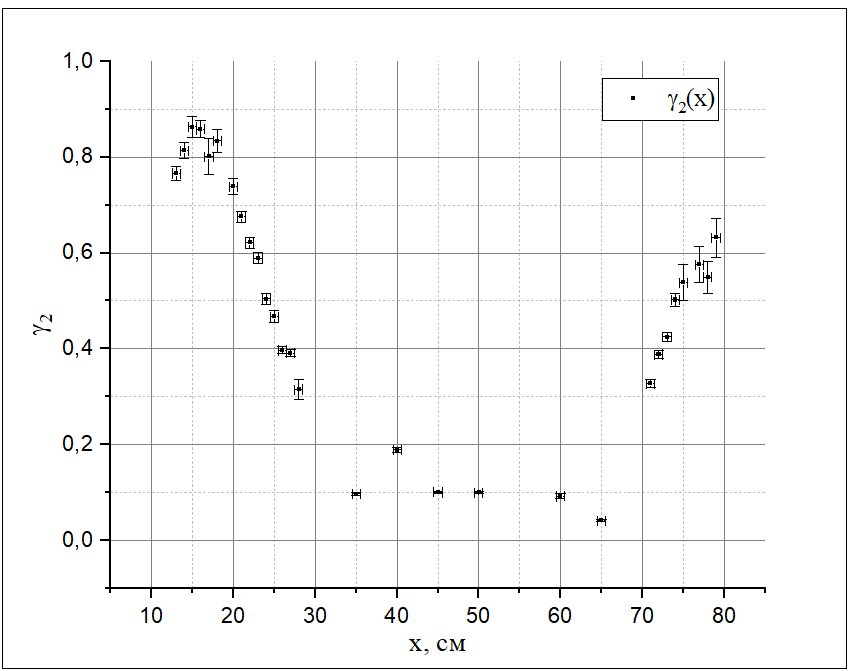
\includegraphics[width =0.8 \linewidth]{gamma2(x).png}
    \captionof{figure}{Зависимость $\gamma_2(x)$}
\end{center}
	
По полученному графику, определив расстояние между максимумами, оценим расстояние $L$ между зеркалами оптического резонатора лазера  и межмодовое расстояние $\Delta\nu$ по формуле (2):
		\begin{equation*}
		L = \frac{2x}{2} = 62,\; L = (62\pm 3) \; \text{см}.
		\end{equation*}
		
		\begin{equation*}
	    \Delta\nu = \frac{c}{2L} = (2,41\pm 0,06)\cdot 10^8 \; \text{Гц}.
		\end{equation*}
		
Определим полуширину $l_{1/2}$ отдельного максимума на половине высоты и рассчитаем диапазон частот $2\Delta F$, в котором происходит генерация продольных мод:
		\begin{equation}
		l_{1/2} \approx 11\; \text{см}, \; 2\Delta F = \frac{2c\sqrt{\ln 2}}{\pi l_{1/2}} \approx 1,45\cdot 10^9 \; \text{Гц}.
		\end{equation}
		
Оценим число генерируемых лазером продольных мод:
		\begin{equation}
		N = 1 + \frac{2\Delta F }{\Delta\nu} \approx 7.
		\end{equation}

\section*{5. Выводы}
	Точки графика рис.4 намного лучше ложатся на прямую, чем точки графика рис.3б. Это связано с хаотически меняющимся направлением линейной поляризации источника. Действительное значение расстояния между зеркалами составляет 65 см, что в пределах $\sigma$ сходится с полученными нами данными. По рис.5 можно предположить, что число мод равно 7.
	
\end{document}

